\documentclass[journal,12pt,twocolumn]{IEEEtran}
\usepackage{amsmath,amsfonts,amssymb,float,gvv,graphicx,enumitem,array,esint}
\bibliographystyle{IEEEtran}
\vspace{3cm}
\title{NCERT Discrete}
\author{Pragnidhved Reddy\\EE23BTECH11050}
\date{}
\parindent 0px
\begin{document}
\maketitle
\newpage
\bigskip
\textbf{Question 11.9.3.18:}\\
 Find the sum to n terms of the sequence $8,88,888,8888$\ldots\\
 \solution \\
 \begin{table}[H]
\centering
\setlength{\extrarowheight}{8pt}
\begin{tabular}{|c|c|c|}\hline
\textbf{Parameter} & \textbf{Value} & \textbf{description}\\ \hline
$x(0)$ & 8 & First term \\ \hline
$x(1)$ & 88 & Second term \\ \hline 
$x(n)$ & $(\sum^{n}_{k=0}8(10)^k)u(n)$ & General term \\ \hline
$S(n)$ & $S(n)=\sum^{n-1}_{k=0}x(k)$ & Sum of n terms \\ \hline
\end{tabular}
\caption{Input parameters}
\label{tab:table1}
\end{table}
 From \eqref{tab:table1}
\begin{align}
\label{eq:1}
 s(n)&=x(n)* u(n)
 \end{align}
 Z transform of general term
 \begin{align}
 X(z)&=\sum_{n=-\infty}^{\infty}(\sum_{k=0}^{n}8(10)^k)u(n)z^{-n}\\[6pt]
 X(z)&=\sum_{n=0}^{\infty}(\sum_{k=0}^{n}8(10)^k)z^{-n}\\[6pt]
 \implies X(z)&=\left(\frac{8z^2}{(z-10)(z-1)}\right) \quad \abs{z}>10
\end{align}
From \eqref{eq:1}, we get
 \begin{align}
 \label{eq:6}
 \implies S(z)&=\left(\frac{8z^2}{(z-10)(z-1)}\right)\left(\frac{1}{z-1}\right)\\[6pt]
 S(z)&=\left(\frac{8z^2}{(z-10)(z-1)^2}\right)\\[6pt]
 s(n)&=\frac{1}{2\pi j}\oint_{c}\frac{8z^2}{(z-10)(z-1)^2}(z^{n-1})dz
 \end{align}
\begin{align}
s(n)&=\frac{1}{2\pi j} \oint_{c} \left(\frac{800z^{n-1}}{81(z-10)}-\frac{8z^{n-1}}{9(x-1)^2}-\frac{152z^{n-1}}{8(z-1)}\right)z^{n-1}dz\\
\notag \implies s(n)&=\lim_{z\to10}\frac{1}{0\displaystyle !\,}\left(\frac{800z^{n-1}}{81}\right)-\lim_{z\to1}\frac{1}{1\displaystyle !\,}\frac{d}{dz}\left(\frac{8z^{n-1}}{9}\right) \\ &~~~~~~~~~~-\lim_{z\to1}\frac{1}{0\displaystyle !\,}\left(\frac{152z^{n-1}}{8}\right)\\
 s(n)&=\left(\frac{8}{81}\right)(10^{n+1}-9n-10)   
\end{align}
\begin{figure}[h!]
    \centering
    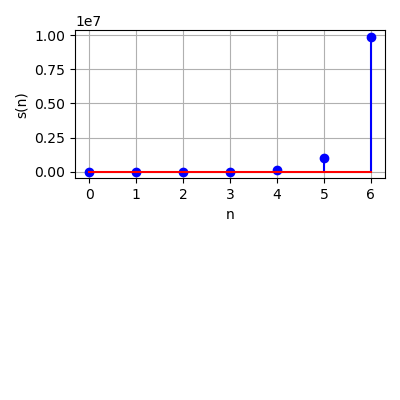
\includegraphics[width=\columnwidth]{figs/plot.png}
    \caption{graph of sum of n terms}
    \label{fig:1}
\end{figure}
 \end{document}
